\section{FOXM1 controls G2-M gene expression through atypical chromatin binding mechanisms}

\subsection{Validation of FOXM1 ChIP-seq data}

The analysis of next generation sequencing (NGS) data is computationally and statistically challenging. Currently there are no benchmarks for data processing methods (read mapping, peak calling \textit{etc.}). Hence false positives/negatives are common problems in experiments, such as ChIP-seq, based on NGS technologies (reviewed in \cite{pepke2009computation}). To confirm the reliability of the FOXM1 ChIP-seq data, vigorous validations were carried out.

\begin{figure}[!h]
    \centering
    \includegraphics[width=0.9\textwidth]{chapter3/figures_foxm1/fig16.pdf}
    \caption[FOXM1 binding at known target genes]{\textbf{FOXM1 binding at known target genes. (A)} known target genes of FOXM1 according to The Transcription Factor Encyclopaedia (\cite{yusuf2012the}). Red colour indicates the genes that are also identified by the FOXM1 ChIP-seq experiment. \textbf{(B)} 52 FOXM1 target genes identified from the microarray analysis (\cite{laoukili2005foxm1}). \textbf{(C)} Snapshots of FOXM1 peak profile at the four well-known target genes.}
    \label{fig:fig16}
\end{figure}

Since many FOXM1 target genes have been discovered in the past, we first checked whether those known target genes were also identified by our FOXM1 ChIP-seq analysis. To this end, we looked into The Transcription Factor Encyclopaedia (\cite{yusuf2012the}), a manually-curated transcription factor database, and found 37 potential target genes of FOXM1 according to previous wet lab experimental evidence. 7 out of 37 genes were bound by FOXM1 based on our ChIP-seq data (\textbf{Figure \ref{fig:fig16}A}). In addition, an early study used microarray analysis and revealed 52 genes that were upregulated when FOXM1 was overexpressed in U2OS cells (\cite{laoukili2005foxm1}). 17 out of 52 genes were bound by FOXM1 (\textbf{Figure \ref{fig:fig16}B}). Note that the target genes from the database and the microarray analysis include both direct and indirect targets of FOXM1, while the genes identified from the ChIP-seq are more likely to be direct FOXM1 targets. In particular, the previously well-established FOXM1 targets \textit{CCNB1, CDC25B, CENPF} and \textit{PLK1} were all present in our FOXM1 ChIP-seq data (\textbf{Figure \ref{fig:fig16}C}) (\cite{laoukili2005foxm1,wang2005forkhead}).

Having confirmed that some known target genes were successfully identified by our FOXM1 ChIP-seq experiment, we next picked different peaks from the ChIP-seq data and used locus-specific ChIP-qPCR to validate the FOXM1 binding at these regions in U2OS cells. FOXM1 binding peaks were ranked by fold enrichment over $\lambda_{local}$, and thirteen peaks with different enrichments were selected. Eleven of these regions showed at least 4 fold enrichment over a non-specific IgG control (\textbf{Figure \ref{fig:fig17}A}).

To further confirm that the ChIP-seq derived peaks were genuine FOXM1 peaks, ChIP experiments were performed on U2OS cells using the FOXM1 antibody after transfection with siRNA against either GAPDH or FOXM1. The FOXM1 binding signal at three tested regions were significantly reduced after the FOXM1 knockdown (\textbf{Figure \ref{fig:fig17}B}), suggesting that the binding signals at those regions represented real FOXM1 binding.

Since the FOXM1 binding events identified from the ChIP-seq analysis were from cells which are at the G2 and M phases, we next checked whether FOXM1 binds to its target genes at other stages of the cell cycle. To this end, U2OS cells were synchronised at the G1/S boundary by a double thymidine block, and cells were released from the thymidine block to allow them to enter the cell cycle. Then FOXM1 ChIP experiments were performed when cells were accumulated at different cell cycle phases: 5 hours after the release (S phase) and 10 hours after the release (G2/M phase). The binding of FOXM1 to four tested target genes happened as early as the G1/S boundary (\textbf{Figure \ref{fig:fig17}C}, 0h time point). Interestingly, the binding of FOXM1 remained relatively constant throughout the different cell cycle stages (\textbf{Figure \ref{fig:fig17}C}), which is consistent with previous findings (\cite{laoukili2008activation}).

\begin{figure}[!h]
    \centering
    \includegraphics[width=0.9\textwidth]{chapter3/figures_foxm1/fig17.pdf}
    \caption[ChIP-qPCR validation on selected FOXM1 peaks]{\textbf{ChIP-qPCR validation on selected FOXM1 peaks. (A)} 13 randomly selected FOXM1 peaks were tested by ChIP-qPCR in U2OS cells using a FOXM1 antibody and a non-specific IgG control antibody. Fold enrichment over the IgG control is indicated above the bar. The error bars represent the standard deviations from three independent experiments. \textbf{(B)} Examination of FOXM1 binding by ChIP-qPCR on three FOXM1 peaks after FOXM1 knockdown. U2OS cells were transfected with 20 nM siRNA against either GAPDH or FOXM1, and cells were collected 48 hours after the transfection. ChIP experiments were performed using a FOXM1 antibody. The error bars represent the standard deviations from two independent experiments. \textbf{(C)} The promoter binding of FOXM1 at different cell cycle stages. U2OS cells were collected at the indicated time points after the release from a double thymidine block. ChIP experiments on the indicated loci were performed using a FOXM1 antibody. The error bars represent the standard deviations from either three independent experiments (the \textit{CKS1, CENPF} and \textit{CCNB1} loci) or two independent experiments (the \textit{CCNG2} locus).}
    \label{fig:fig17}
\end{figure}

In summary, our FOXM1 ChIP-seq data is consistent with previous findings about FOXM1. Most of the peaks validated from the ChIP-seq data have real FOXM1 binding. The binding of FOXM1 at a subset of tested regions happens at the early stages of the cell cycle and remain relatively constant during the cell cycle. These findings indicate that the quality of our FOXM1 ChIP-seq data is good.

\pagebreak

\subsection{FOXM1 regulates a large array of late cell cycle genes}

After confirming the reliability of the FOXM1 ChIP-seq data, the biological functions and the molecular mechanisms of FOXM1 binding were investigated.

FOXM1 is known as a cell cycle regulator, and it is required for proper G2-M transition and chromosome segregation (\cite{laoukili2005foxm1,wang2005forkhead}). To establish whether more of the FOXM1 target genes were also involved in G2-M cell cycle regulation and to discover potential novel functions of FOXM1, the ChIP-seq derived peaks were analysed by the \underline{G}enomic \underline{R}egions \underline{E}nrichment of \underline{A}nnotations \underline{T}ool (GREAT), an analytical tool of gene ontology (\cite{mclean2010great}). Previous gene ontology methods only take the proximal binding events into consideration, simply assign one binding event to its nearest gene, and use gene-based tools to perform the functional interpretation (\cite{huang2009bioinformatics}). Unlike the traditional methods, GREAT is a peak/region-based analysis, which is more similar to the nature of the transcription factor ChIP-seq data. In GREAT, each gene is first given a basal domain which is from 5 kb upstream to 1 kb downstream of the TSS of that gene. Then the basal domain is extended upstream and downstream to the basal domains of its neighbouring genes within 1 Mb. The resulting basal plus extension domain is denoted as the regulatory domain of the gene, and any peaks that fall into the regulatory domains will be assigned to the particular genes (\textbf{Figure \ref{fig:fig18}A}). Only enriched terms that satisfy both binomial and hypergeometric tests are returned. In this way, GREAT is able to associate a peak and its potential target genes together even if they are far away. This approach significantly improves the functional interpretation of the transcription factor binding events (\cite{mclean2010great}).

\begin{figure}[!h]
    \centering
    \includegraphics[width=0.9\textwidth]{chapter3/figures_foxm1/fig18.pdf}
    \caption[Gene ontology analysis of FOXM1 peaks by GREAT]{\textbf{Gene ontology analysis of FOXM1 peaks by GREAT. (A)} The basal plus extension rules of GREAT. The arrow indicates the transcription start site of each gene. The thick line and the thin line represent the basal (-5 kb plus +1 kb relative to the TSS) and the extended domain (up to 1 Mb) respectively. The whole regulatory domain for each gene is shown as a bracketed line in matched colour. \textbf{(B)} Histogram showing number of associated genes per peak. \textbf{(C, D, E and F)} Top 20 terms of Biological Process \textbf{(C)}, top 20 terms of Cellular Component \textbf{(D)}, all terms of Mouse Phenotype \textbf{(E)}, and top 20 terms of MSigDB Pathway \textbf{(F)}. The P-value, FDR, and fold enrichment based on binomial distribution are also given.}
    \label{fig:fig18}
\end{figure}

By the use of GREAT, all FOXM1 peaks were assigned to at least one gene per peak, and 100 peaks were assigned to two genes per peak (\textbf{Figure \ref{fig:fig18}B}). GREAT returned 91 enriched terms for Biological Process, 33 for Cellular Component, 9 for Mouse Phenotype, and 35 for MSigDB Pathway (\textbf{Figure \ref{fig:fig18}C-F}). Consistent with the previous notion that FOXM1 regulates the G2-M cell cycle transition, the majority of the Biological Process terms were related to cell cycle, mitosis, and chromosome segregation (\textbf{Figure \ref{fig:fig18}C}). In addition, most enriched terms of Mouse Phenotype and MSigDB Pathway were also linked to M phase and cell cycle, and many enriched Cellular Component terms, such as spindle, kinetochore, and centrosome, were critical for mitosis (\textbf{Figure \ref{fig:fig18}C}). In addition, there were also a few enriched terms which were not directly linked to cell cycle, such as DNA packaging, DNA conformation change and free ubiquitin chain polymerisation, although the P-values were not as significant as those cell cycle related terms (\textbf{Figure \ref{fig:fig19}}). This indicates that FOXM1 might also play some regulatory roles in those processes. Interestingly, many genes within the non-cell cycle terms are also G2-M transition regulators, indicating that some terms which are not directly linked to cell cycle are the biological processes associated with the mitotic cell cycle.

\begin{figure}[!h]
    \centering
    \includegraphics[width=0.8\textwidth]{chapter3/figures_foxm1/fig19.pdf}
    \caption[Enriched terms of Biological Process for FOXM1 peaks by GREAT]{\textbf{Enriched terms of Biological Process for FOXM1 peaks by GREAT.} An expansion of Figure 18C, showing all enriched terms from Biological Process which are sorted by -log\sub{10}P-value.}
    \label{fig:fig19}
\end{figure}

Given that most FOXM1 target genes were related to the cell cycle, especially mitosis, we then checked the expression patterns of all 362 FOXM1-bound genes assigned by GREAT throughout the cell cycle. To this end, we took advantage of a recent microarray study in HeLa cells after release from a double thymidine block, which examined the gene expression patterns in different cell cycle stages (\cite{sadasivam2012the}). Most of FOXM1-bound genes exhibited strong cell cycle-dependent expression, with peak activities when cells entered into G2 and M phase (\textbf{Figure \ref{fig:fig20}A}). This is consistent with the gene ontology analysis and suggests that FOXM1 has a role in controlling the temporal expression of genes in the G2 and M phases.

\begin{figure}[!h]
    \centering
    \includegraphics[width=0.9\textwidth]{chapter3/figures_foxm1/fig20.pdf}
    \caption[Expression patterns of FOXM1 bound genes throughout the cell cycle]{\textbf{Expression patterns of FOXM1 bound genes throughout the cell cycle. (A) Left,} heatmap of expression levels (represented by Z-score) of FOXM1 bound genes at the indicated time points after the release from a double thymidine block. The three replicates of each time point are shown. \textbf{Right,} average expression levels of FOXM1 bound genes at different cell cycle stages. This was done by Dr. Namshik Han. \textbf{(B)} Overlap between the 422 genes which give a mitotic phenotype when depleted (\cite{neumann2010phenotypic}) and 362 FOXM1 target genes assigned by GREAT. The overlapping genes are shown at the bottom. P-value was calculated by Fisher's exact test.}
    \label{fig:fig20}
\end{figure}

To further address the importance of FOXM1 in controlling late cell cycle events, we looked into the validation screen database of the Mitocheck consortium (\cite{neumann2010phenotypic}). This consortium carried out phenotypic profiling with a siRNA library targeting \textasciitilde 21,000 human protein coding genes using live-cell imaging. The validated database contained 422 genes which gave at least one mitotic phenotype upon knockdown, and 34 of them overlapped with the 362 FOXM1-bound genes (\textbf{Figure \ref{fig:fig20}B}). This strongly suggests that FOXM1 regulates a subset of genes which are important for mitosis.

Since the number of binding events of many transcription factors far exceeds their known or possible target genes, a large number of their binding events have no apparent biological functions (reviewed in \cite{macquarrie2011genome-wide}). To investigate whether the FOXM1 binding events are functional, we tested the effect of FOXM1 depletion on the expression kinetics of ten of its target genes. U2OS cells were released from a double thymidine block and allowed to enter the G2 and M phases (\textbf{Figure \ref{fig:fig10}C}). Total RNA was collected every hour during a period that encompasses the G2 and M phases, and gene expression levels were measured by RT-qPCR. As expected, FOXM1 knockdown resulted in reduced expression levels of known target genes like \textit{CCNB1} and \textit{CENPF} (\textbf{Figure \ref{fig:fig21}}). More importantly, the depletion of FOXM1 also caused reduced expression of other newly identified target genes, albeit the effects on \textit{SKA2} and \textit{CDC20} were marginal (\textbf{Figure \ref{fig:fig21}}).

Interestingly, although the ten target genes tested were all thought to be activated at the G2 and M phases, they showed different kinetics of expression (\textbf{Figure \ref{fig:fig21}}, blue lines). For example, the expression of \textit{CCNF, CENPA} and \textit{CDC20} peaked at 10, 11, and 12 hours respectively after the release from double thymidine block; the level of \textit{CCNB1} increased significantly when cells entered G2 phase and the expression was maintained throughout the G2 and M phases, whereas \textit{CCNF, FZR1,} and \textit{KPNA2} expression reduced after their peak time and gradually declined to near basal level; the expression of \textit{NUCKS1} did not fluctuate during the cell cycle (\textbf{Figure \ref{fig:fig21}}). This indicates that the FOXM1 regulates a set of genes which exhibit different expression kinetics. In addition, most target genes have reduced levels of expression upon FOXM1 knockdown, but they still possess a certain degree of oscillation but at a lower amplitude (\textbf{Figure \ref{fig:fig21}}, red lines), suggesting that the remaining residue of FOXM1 or some compensatory mechanism could still control the oscillation of gene expression.

\begin{figure}[!h]
    \centering
    \includegraphics[width=0.9\textwidth]{chapter3/figures_foxm1/fig21.pdf}
    \caption[The expression pattern of FOXM1 target genes in the G2 and M phases of the cell cycle upon FOXM1 depletion]{\textbf{The expression pattern of FOXM1 target genes in the G2 and M phases of the cell cycle upon FOXM1 depletion.} U2OS cells were transfected with either a non-targeting siRNA or siRNA against FOXM1. Then cells were synchronised by double thymidine block and released into fresh media to allow the progression to G2 and M phase. Total RNA was collected at indicated time points after the release, and the mRNA levels were measured by RT-qPCR using gene-specific primers. The expression levels were first normalised by the 12h time point of the siCon sample, and then normalised by the expression of the reference gene \textit{HMBS}. The error bars represent standard deviations from two independent experiments. The P-value was calculated using a t-test. * and ** represent P<0.05 and P<0.01, respectively.}
    \label{fig:fig21}
\end{figure}

In summary, the FOXM1 ChIP-seq data suggests that it controls the expression of a large array of cell cycle regulated genes which are critical for mitosis and chromosome segregation. This is consistent with the previous notion of FOXM1 that it is one of the master regulators of G2-M cell cycle events (\cite{laoukili2005foxm1}). Our data has added a large number of novel target genes to the FOXM1 regulome.

\subsection{The CHR motif, not the canonical Forkhead motif, is enriched in the FOXM1 cistrome}

Having confirmed that FOXM1 controls the transcription of a large array of G2-M genes, the mechanism of the regulation was investigated. FOXM1 is a transcription factor, and transcription factors can make direct contacts with DNA. Therefore, it is logical to assume that FOXM1 regulates its target genes by directly binding to the DNA within the regulatory regions of its target genes.

To test this hypothesis, a \textit{de novo} motif discovery program, HOMER (\cite{heinz2010simple}), was used to find the overrepresented DNA sequences within 200 bp centred on the summits of FOXM1 ChIP-seq derived peaks. Since FOXM1 belongs to the Forkhead transcription factor family, we expected to find motifs similar to the Forkhead consensus RYMAAYA, as this was the case in the ChIP-seq studies of other Forkhead transcription factors like FOXO3 (\textbf{Figure \ref{fig:fig14}C}), FOXK2 (\cite{ji2012the}), FOXA1 (\cite{hurtado2011foxa1}), and FOXP3 (\cite{katoh2011foxp3}). However, the motif discovery failed to detect overrepresentation of canonical Forkhead consensus. Instead, two other motifs, the CCAAT-box motif and the CHR motif, were significantly enriched within the FOXM1 peaks (\textbf{Figure \ref{fig:fig22}A}).

The finding that the canonical Forkhead consensus RYMAAYA is not enriched within the FOXM1-bound regions is quite surprising. To confirm the reliability of this discovery, a traditional motif finding program MEME (\cite{bailey1994fitting}) was used to perform \textit{de novo} motif discovery from the ChIP-seq derived peaks of FOXM1. In agreement with HOMER, the top two motifs found by MEME were also the CCAAT-box motif and the CHR motif (\textbf{Figure \ref{fig:fig22}B}). In addition, a GC-rich motif was also returned by MEME, but not by HOMER. The reason that HOMER did not find the GC-rich motif was probably because HOMER, by default, randomly chooses background sequences whose GC-content is similar to the target sequences from the interrogated genome. Since most FOXM1 binding peaks are located within CpG islands (77\%), the background will be chosen from GC-rich regions from the genome as well. Therefore, the GC-rich motif might not be enriched in the FOXM1 binding regions compared to the background sequences. Indeed, when randomly chosen background sequences from the genome without the consideration of GC-content are used, HOMER also returned a GC-rich motif like MEME (data not shown).

\begin{figure}[!h]
    \centering
    \includegraphics[width=0.9\textwidth]{chapter3/figures_foxm1/fig22.pdf}
    \caption[Motif discovery and analyses of FOXM1 peaks]{\textbf{Motif discovery and analyses of FOXM1 peaks. (A)} Two significantly enriched motifs returned by HOMER. The P-value was calculated based on the hypergeometric distribution. The percentage of target sequence and background sequence containing the indicated motif are also shown. Motif alignment against a custom collection of transcription factor motif database (\cite{heinz2010simple}) is shown in the \textbf{Best match} column. \textbf{(B)} Three significantly enriched motifs returned by MEME. The E-value and the percentage of target sites containing the motif are shown. The E-value returned by MEME is an estimate of the number of motifs one would expect to find by chance if the target sequences are shuffled. \textbf{(C)} Number of FOXM1 peaks or background sequence containing the sequence TAAACA. \textbf{(D)} The frequency of occurrence of the indicated motifs around the FOXM1 summits. FOXM1 ChIP-seq derived peaks were aligned by their summits, and a region of -500 bp and +500 bp relative to the summit was selected. Motif frequency was counted at every 10 bp bin. For the Forkhead site, the RYMAAAYA sequence was searched; for the NFYA motif and the CHR motif, the matrix shown in \textbf{(A)} was searched.}
    \label{fig:fig22}
\end{figure}

Since the hexamer sequence TAAACA was previously shown to be bound by FOXM1 \textit{in vitro} by selection and amplification of binding sites (\cite{korver1997the}), we searched the occurrence of the motif TAAACA with the 200 bp DNA sequences centred on the 270 FOXM1 summits. For parallel comparison, a random set of 270 sequences 200 bp in length and with a similar genomic distribution to the FOXM1 270 peaks were chosen from the genome as background sequences. The motif search showed that there were, indeed, only 25 FOXM1 peaks containing at least one TAAACA motif, but there were also 25 background sequences containing the motif (\textbf{Figure \ref{fig:fig22}C}). This clearly indicates that the presence of the TAAACA motif within the FOXM1 peaks is random, and there is no enrichment of this motif.

The summit (highest point where tags pile up) of the peak normally reflects the crosslinked point, hence the protein-DNA interaction site, and the most overrepresented DNA motif is generally believed to be the sequence bound by the protein. Therefore, in a typical ChIP- seq data, the enriched DNA motifs bound by the protein are regularly more frequent near the summit than the surrounding area (\cite{zhang2008model-based}). To further investigate whether the canonical Forkhead motif might be bound by FOXM1, the frequency of the motif occurrence around the FOXM1 summits was counted. Consistent with the motif search, the Forkhead motif is dispersed throughout the regions. In contrast, both the CCAAT-box motif and the CHR motif occurred much more frequently near the summit, although their frequency curves did not peak at the exact summit point (\textbf{Figure \ref{fig:fig22}D}). The CHR motif was even more frequent than the CCAAT-box motif at these locations.

\begin{figure}[!h]
    \centering
    \includegraphics[width=0.9\textwidth]{chapter3/figures_foxm1/fig23.pdf}
    \caption[FOXM1 binding at different regions of the PLK1, CCNB2 and AURKB promoters]{\textbf{FOXM1 binding at different regions of the \textit{PLK1}, \textit{CCNB2} and \textit{AURKB} promoters.} ChIP-qPCR analysis of FOXM1 binding at different regions on the promoter of its target genes. ChIP was performed in U2OS cells using a FOXM1 antibody. A non- specific IgG antibody was also included as a control. Primers are indicated as arrows. The Forkhead consensus sequences (FC) and their positions are shown. Error bars of the \textit{PLK1} and \textit{CCNB2} loci represent the standard deviations from two independent experiments. Error bars of the \textit{AURKB} locus is the standard deviation from two technical replicates of qPCR in one experiment.}
    \label{fig:fig23}
\end{figure}

To experimentally validate that the Forkhead consensus is not enriched in FOXM1- bound peaks, three well-defined FOXM1 target genes, \textit{CCNB2, PLK1 and AURKB} were chosen, and primers were designed to target different regions of their promoters which contain both the Forkhead consensus and the CHR motif (\textbf{Figure \ref{fig:fig23}}). Then FOXM1 ChIP experiments were performed, and the binding at those regions was detected using qPCR. Consistent with previous results, the binding signals of FOXM1 were highest around the transcription start sites of those genes, where the CHR motif is located (\textbf{Figure \ref{fig:fig23}}). Although some binding was able to be detected at the regions where the Forkhead consensus located comparing to a non-specific IgG IP, the signals were at a low level (\textbf{Figure \ref{fig:fig23}}), possibly due to incomplete sonication of the DNA surrounding the binding locus. This reinforces the motif discovery results from an experimental point of view.

In summary, the canonical Forkhead consensus RYAAAYA motif is not enriched in the FOXM1 cistrome. Instead, the CCAAT-box, which has been shown bound by the transcription factor NF-Y, and the CHR motif are enriched in the FOXM1-bound regions. Moreover, the CCAAT-box and the CHR motif occur more frequently near the summits than the surrounding area, indicating FOXM1 is actually associated with these two motifs in vivo. Therefore, it seems that the data do not support our original assumption that FOXM1 regulates target genes by directly binding the DNA through motifs generally associated with the Forkhead protein binding in their regulatory elements.

\subsection{FOXM1 does not directly bind to the CHR motif}

Given that the CCAAT-box and the CHR motif are overrepresented within the FOXM1- bound regions, we next began to investigate whether FOXM1 can directly bind to either of these DNA motifs.

We first reasoned that the CCAAT-box has been shown bound by the transcription factor NF-Y (reviewed in \cite{mantovani1999the}), and this motif is prevalent in the promoters of many cell cycle genes, not specific for G2-M genes. It is unlikely that FOXM1 can directly bind to this DNA sequence (see below).

We then noticed that the CHR motif, to some extent, resembles the canonical Forkhead consensus: both of them are AT-rich DNA motifs. Previous studies suggest that FOXM1 binds to the canonical Forkhead consensus at an extremely low affinity (\cite{freddie2007functional,littler2010structure}). Therefore, it was possible that FOXM1 can somehow directly bind to the CHR motif to regulate the transcription of its target genes.

To check whether this is the case, band shift experiments were performed using a 6$\times$His and FLAG-tagged FOXM1 DNA-binding domain purified from bacteria. We first tested the interaction between the FOXM1 DNA-binding domain and the DNA sequence from the \textit{PLAC8} locus, which contains a canonical Forkhead consensus GTAAACA (\textbf{Figure \ref{fig:fig24}A}). FOXK2 and FOXO3 DNA-binding domains which were purified from bacteria in a similar way were used as positive controls (\textbf{Figure \ref{fig:fig24}B}). When added at 90 nM concentrations, clear FOXK2-DNA and FOXO3-DNA complexes were observed (\textbf{Figure \ref{fig:fig24}C}, lanes 2 and 3), but a FOXM1-DNA complex could not be detected (\textbf{Figure \ref{fig:fig24}C}, lane 4). With the concentration of FOXM1 DNA-binding domain increased to 900 nM, a weak protein-DNA complex was detected when the DNA sequences from the wild-type \textit{PLAC8} or \textit{MMP9} loci was used (\textbf{Figure \ref{fig:fig24}D}, lanes 2 and 5). After the addition of FLAG antibody, the intensity of protein-DNA complex significantly reduced, indicating that the complex was genuine FOXM1-DNA (\textbf{Figure \ref{fig:fig24}D}, lanes 3 and 6). However, a super-shift was not observed, presumably due to the unstable interactions of the FLAG antibody/FOXM1/DNA ternary complex. In addition, the FOXM1-DNA interaction was indeed a specific binding between FOXM1 and the canonical Forkhead consensus, because when the GTAAACA sequence in the wild-type \textit{MMP9} promoter was mutated to GTAAAAA, FOXM1 failed to form a complex with the mutated DNA sequence (\textbf{Figure \ref{fig:fig24}D}, lanes 8 and 9). More importantly, when a DNA sequence from the wild-type \textit{CCNB1} promoter, which contains the CHR motif, was added to the reactions, the FOXM1-DNA complex was undetectable (\textbf{Figure \ref{fig:fig24}D}, lanes 11 and 12).

The bandshift experiments suggest that FOXM1 cannot directly bind to the CHR motif. However, in this kind of experiment, only purified FOXM1 DNA-binding domain was tested. There are still possibilities that FOXM1 can make direct interaction with the CHR motif: (1) the full-length FOXM1 protein can bind to the CHR motif; (2) post-translational modifications might assist its binding to the CHR motif; (3) interactions with other proteins switch its binding specificity making FOXM1 directly bind to the CHR motif, a common mechanism utilised by many transcription factors to enhance specificity (\cite{siggers2011non-dna-binding,slattery2011cofactor}).

\begin{figure}[!h]
    \centering
    \includegraphics[width=0.9\textwidth]{chapter3/figures_foxm1/fig24.pdf}
    \caption[Bandshift experiments of \textit{in vitro} DNA-binding of Forkhead proteins]{\textbf{Bandshift experiments of \textit{in vitro} DNA-binding of Forkhead proteins. (A) Left,} schematic view of the Forkhead proteins used in the experiments. The numbers on the protein schematics delineate the amino acids at the start and the end of the fragments relative to the full-length protein. The position of the Forkhead DNA binding domain (FKH) is also indicated. \textbf{Right,} the DNA sequences from indicated loci used in the experiments. The motifs within the DNA sequences are underlined, and the mutation in the MMP9 locus-derived sequence is shown in red. \textbf{(B)} The Coomassie staining of the gels which contain purified DNA-binding domain of FOXK2 (left), FOXO3 and FOXM1 (right). Varying amounts of BSA and elutes of different proteins were run as indicated. The Molecular weight of the marker band is shown. Asterisks indicate possible non-specific proteins pulled down during the His tag purification. \textbf{(C)} The binding between the DNA sequence from \textit{PLAC8} locus and the DNA-binding domains of indicated Forkhead proteins. Proteins were added at 90 nM concentration. The binding reactions were run on a non-denaturing poly-acrylamide gel. The free DNA and the protein-DNA complexes are indicated by arrows. \textbf{(D)} The interaction between FOXM1 and DNA sequences from the indicated loci. The FOXM1 DNA- binding domain was added at 900 nM concentration. A FLAG antibody was added where indicated. The free DNA and the FOXM1-DNA complexes are indicated by arrows.}
    \label{fig:fig24}
\end{figure}

To investigate these possibilities, an \textit{in vitro} DNA pull-down assay was carried out. In this experiment, the wild-type DNA sequence from the \textit{CCNB1} promoter or various mutated versions were coupled with a biotin tag. The biotin-tagged DNA sequence was bound to streptavidin-linked magnetic beads, followed by the incubation with the cell extract from U2OS cells. After washing off the non-specific binding proteins, elutes were analysed using SDS-PAGE, and the bound proteins were detected by western blot using specific antibodies. A DNA sequence from a part of the luciferase gene was used as a negative control (\textbf{Figure \ref{fig:fig25}A}). The \textit{CCNB1} promoter sequence used in this experiment contains three well-defined motifs: the CCAAT-box motif which is bound by the transcription factor NF-Y, a CDE-like GC-rich motif which is important for the transcription of some, if not all, G2-M genes, and the CHR motif (\textbf{Figure \ref{fig:fig25}B}). Each of these was mutated individually and in a combined manner to assess the potential impact on FOXM1 binding.

\begin{figure}[!h]
    \centering
    \includegraphics[width=0.9\textwidth]{chapter3/figures_foxm1/fig25.pdf}
    \caption[\textit{In vitro} DNA pull-down assay to investigate FOXM1-DNA interactions]{\textbf{\textit{In vitro} DNA pull-down assay to investigate FOXM1-DNA interactions. (A)} Schematic view of linking biotin-tagged DNA sequence to the streptavidin conjugated magnetic beads to generate the bait for the pull-down experiment. \textbf{(B)} The DNA sequence of \textit{CCNB1} promoter used in the pull-down experiments. The two CCAAT-boxes, the GC-rich, and the CHR motifs are shown, and the rest part of the promoter is omitted. The arrow indicates the transcription start site according to RefSeq. \textbf{(C)} DNA pull-down experiment to test the DNA-binding of FOXM1 and NF-YA. U2OS cell extracts were incubated with the indicated DNA sequences which were linked to the magnetic beads. The precipitated material was immunoblotted (IB) with the indicated antibodies. \enquote{$\Delta$} indicates the mutation of the motif, and \enquote{-} indicates the deletion of the motif. A fragment of DNA from the luciferase coding sequence was used as control.}
    \label{fig:fig25}
\end{figure}

As expected, the transcription factor NF-YA was able to bind the wild-type \textit{CCNB1} promoter sequence (\textbf{Figure \ref{fig:fig25}C}, lane 4). When the GC-rich or CHR motif was mutated, it still bound to the DNA sequence (\textbf{Figure \ref{fig:fig25}C}, lanes 5, 6 and 7), but lost its binding after the CCAAT-box motif was mutated (\textbf{Figure \ref{fig:fig25}C}, lanes 8 and 9). This is consistent with previous research showing that NF-YA bound to the CCAAT-box motif, and this binding was independent of the GC-rich and CHR motifs (\cite{müller2012the}). In contrast, the binding signals of FOXM1 remained relatively constant among the wild-type and all mutant promoter sequences (\textbf{Figure \ref{fig:fig25}C}, lanes 4 to 9), and the binding levels to the wild-type \textit{CCNB1} promoter sequence was very similar to the control DNA sequence (\textbf{Figure \ref{fig:fig25}C}, lane 3). In the absence of any DNA, no binding signal was detected (\textbf{Figure \ref{fig:fig25}C}, lane 2), indicating that the observed FOXM1 binding was due to the interaction with DNA, not the beads. Therefore, it seems that the affinity of FOXM1 binding to the \textit{CCNB1} promoter sequence is comparable to its non-specific DNA interaction. We are unable to observe sequence-specific binding of FOXM1 or any particular roles of the CHR motif in this binding.

In summary, FOXM1 can directly bind to the canonical Forkhead consensus \textit{in vitro}, even though the Forkhead consensus is not enriched in the ChIP-seq derived FOXM1 peaks. The affinity of FOXM1 for the Forkhead consensus is extremely low, but the interaction is still specific, because a single nucleotide mutation of the Forkhead consensus results in the loss of binding. However, in the in vitro experiments, we have found no evidence that FOXM1 binds to the DNA sequences it occupies \textit{in vivo}. It is therefore likely that a proper genomic context and/or the association with other factors are required for the FOXM1-DNA binding.

\subsection{The DREAM complex and the transcription factor NF-Y do not significantly contribute to FOXM1 DNA binding}

Since FOXM1 fails to make stable contacts with the CCAAT-box and the CHR motifs \textit{in vitro}, we next investigate how these two motifs recruit FOXM1 to the DNA in the cells, and how FOXM1 applies its regulatory roles via them.

The CCAAT-box motif is a NF-Y binding site. Although a previous study suggests that LIN54 can directly bind to the CHR motif \textit{in vitro}, due to technical difficulties of getting recombinant LIN54 protein \textit{in vitro}, the evidence is not convincing (\cite{schmit2009lin54}). On the other hand, a most recent study has demonstrated that the cell cycle regulatory complexes DREAM and MMB require an intact CHR to bind the promoter of many cell cycle genes (\cite{müller2012the}). Therefore, it is reasonable to speculate that either NF-Y or DREAM/MMB recruits FOXM1 to the DNA.

To test this hypothesis, GFP-tagged FOXM1B or FOXM1C isoform were transfected into HEK293 cells, and co-immunoprecipitation was performed using an anti-GFP antibody. The NF-Y is a trimeric transcription factor containing NF-YA, NF-YB, and NF-YC, with NF-YA being the direct DNA-binding subunit, and all three subunits are required for the binding to CCAAT-box (\cite{sinha1996three}). Here, we used NF-YA as a representation of the NF-Y transcription factor. LIN9 and LIN37 were used to represent the MuvB core complex. Clear interactions between both FOXM1 isoforms and LIN9/LIN37 were observed (\textbf{Figure \ref{fig:fig26}A}). The MMB-specific subunit B-MYB was also co-immunoprecipitated with the two FOXM1 isoforms (\textbf{Figure \ref{fig:fig26}A}). However, we were unable to detect interactions of FOXM1 with either of the DREAM-specific subunits E2F4 and p130 (\textbf{Figure \ref{fig:fig26}A}), indicating that FOXM1 does not form stable complex with the DREAM proteins. This is in agreement with the previous findings that the DREAM complex is only present in quiescent cells, while FOXM1 is only expressed in proliferating cells (\cite{litovchick2007evolutionarily,korver1997the}). Similarly, no detectable interactions between the two FOXM1 isoforms and NF-YA could be observed (\textbf{Figure \ref{fig:fig26}A}).

The co-immunoprecipitation indicated that the DREAM complex and the transcription factor NF-Y might not contribute to the DNA-binding of FOXM1. To further confirm these findings, FOXM1 binding to several promoter regions was measured by ChIP-qPCR in U2OS cells after the transfection with a non-targeting siRNA or siRNAs against either E2F4 or NF-YA. Consistent with the negative Co-IP data, knockdown of E2F4 or NF-YA did not significantly change the binding of FOXM1 (\textbf{Figure \ref{fig:fig26}B}).

\begin{figure}[!h]
    \centering
    \includegraphics[width=0.9\textwidth]{chapter3/figures_foxm1/fig26.pdf}
    \caption[FOXM1 interacts with the MMB complex, but not the DREAM complex or NF-Y]{\textbf{FOXM1 interacts with the MMB complex, but not the DREAM complex or NF-Y. (A)} Co-immunoprecipitation of two FOXM1 isoforms with the DREAM/MMB complexes and NF-YA. Plasmids encoding GFP tagged FOXM1B or FOXM1C were transfected into HEK293 cells, and the protein complexes were precipitated with an anti-GFP antibody. The immunoprecipitations were blotted (IB) with indicated antibodies. These experiments were done by Dr. Gerd Muller. \textbf{(B)} ChIP experiments of FOXM1 after the knockdown of E2F4 or NF-YA. U2OS cells were transfected with 20 nM of the indicated siRNAs. 48 hours after the transfection, ChIP experiments were performed using a FOXM1 or non-specific IgG antibody. Error bars represent the standard deviations from two independent experiments. \textbf{(C)} FOXM1 and NF-YA ChIP experiments after the overexpression of either wild-type NF-YA (NFYA WT) or a dominant negative form of NF-YA (NFYA m29). The HEK293 stable cell lines were treated where indicated with 1 $\mu$g/mL doxycycline for 24 hours. ChIP experiments were performed using NF-YA (left) or FOXM1 (right) antibodies. Error bars represent the standard deviation from two independent experiments.}
    \label{fig:fig26}
\end{figure}

In addition, we also investigated the relationship between of NF-Y and FOXM1 DNA binding by using HEK293 stable cell lines which expresses either wild-type NF-YA or a dominant-negative NF-YA (NF-YA m29) under the control of a tetracycline-inducible CMV promoter (\cite{tiwari2011a}). The dominant-negative form of NF-YA is unable to bind DNA, and will interfere with the endogenous NF-YA DNA binding when overexpressed (\cite{mantovani1994dominant}). FOXM1 ChIP experiments were performed and its DNA binding was measured by qPCR with or without the overexpression of the wild-type NF-YA or the dominant negative form of NF-YA. The overexpression of the dominant negative form of NF-YA indeed resulted in a reduced overall binding of NF-YA when a NF-YA antibody was used in the ChIP experiments (\textbf{Figure \ref{fig:fig26}C}, left). However, no accompanying decrease of FOXM1 binding was observed (\textbf{Figure \ref{fig:fig26}C}, right), which is in agreement with the siRNA experiments mentioned before. Similarly, wild-type NF-YA overexpression resulted in an slightly increase in NF-YA binding to the tested promoter regions but had little effect on FOXM1 binding (\textbf{Figure \ref{fig:fig26}C}).

In summary, we were unable to detect stable interactions between FOXM1 and either the DREAM complex or NF-YA. More importantly, knockdown of the DREAM components and NF-YA or overexpression of a dominant-negative form of NF-YA hardly changed the ChIP signals of FOXM1, indicating that they do not contribute greatly to FOXM1 chromatin binding \textit{in vivo}. Hence the over-representation of the CCAAT-box motif is probably due to its common co-occurrence with the CHR motif in the promoter of G2-M genes (\cite{müller2012the}). The interactions of FOXM1 with the MuvB core proteins and the MMB-specific protein B-MYB were clearly detected, indicating the MMB complex is likely to play important role on FOXM1 DNA binding.

\subsection{The CHR motif recruits FOXM1 to chromatin and is important for FOXM1-mediated transcriptional activation}

Having confirmed that the DREAM complex and NF-YA hardly contribute to FOXM1 chromatin binding, we focused on investigating the potential roles of the CHR motif and the MMB complex on the chromatin binding of FOXM1. To this end, we first started with establishing the importance of the CHR motif in recruiting FOXM1 to its regulatory regions.

Within the 270 FOXM1 peaks, there were 173 peaks (CHR+) which contain the CHR motif. When compared to the rest 97 peaks (CHR-) which do not contain the CHR motif, the average binding signals at the CHR+ peaks were generally higher than those at the CHR- peaks (\textbf{Figure \ref{fig:fig27}A}), indicating that FOXM1 has higher occupancy at regions with CHR motif. Therefore, the mechanisms of the recruitment of FOXM1 to these two categories of peaks might be different.

\begin{figure}[!h]
    \centering
    \includegraphics[width=0.9\textwidth]{chapter3/figures_foxm1/fig27.pdf}
    \caption[The CHR motif plays an important role in recruiting FOXM1 to chromatin]{\textbf{The CHR motif plays an important role in recruiting FOXM1 to chromatin. (A) Left,} boxplot of tags in peaks that contain the CHR motif (CHR+) and peaks that do not contain the CHR motif (CHR-). Peak length was normalised to 1 kb. P- value was calculated by an independent t-test. \textbf{Right,} quantification of average tags around the summits of peaks which have or do not have the CHR motif. Peaks were aligned by their summits, and a region of -1 and +1 kb relative to the summit was selected. Tags were calculated in every 10 bp bin across this region and normalised to tags per 10 million total reads per bin per peak. \textbf{(B) Left,} schematic view of the luciferase construct driven by the wild-type and mutated human \textit{CCNB2} promoters integrated in the HCT116 stable cell line. DNA sequences are shown below, and the motifs (CDE and CHR) are shown in colour. \textbf{Right,} ChIP-qPCR analyses of FOXM1 binding at the transgene regions in the HCT116 stable cell lines. The binding at the transgene regions were normalised to the binding signals at the endogenous \textit{CCNB2} locus (taken as 1). Error bars present the standard deviations from three independent experiments, and the P- values are indicated. These experiments were done by Ms. Marianne Quaas.}
    \label{fig:fig27}
\end{figure}

To check whether an intact CHR motif is required for the FOXM1 chromatin binding, HCT116 stable cell lines were previously generated which have luciferase constructs driven by the wild-type or mutant human \textit{CCNB2} promoters integrated into the genome (\textbf{Figure \ref{fig:fig27}B}, left; \cite{müller2012the}). A triple FLAG tagged FOXM1 was transfected into the stable cell lines, and the binding of FOXM1 to the regions of these transgenes was measured by ChIP-qPCR. FOXM1 was able to bind to the region of the wild-type \textit{CCNB2} promoter driven transgene. However, mutation of the CHR motif abolished the binding of FOXM1. In contrast, mutation of the CDE motif did not significantly affect FOXM1 binding ($p=0.13$) (\textbf{Figure \ref{fig:fig27}B}, right). This indicates that the recruitment of FOXM1 to chromatin is dependent on the CHR motif.

Given that the CHR motif is critical for the FOXM1 chromatin binding, we next checked whether it is also important for the FOXM1-mediated gene activation. Luciferase constructs driven by the wild-type or mutant human \textit{CCNB1} promoter and the \textit{FOXM1} expression plasmid were co-transfected into U2OS cells, and the luciferase activities were measured to assess the gene activation by FOXM1. Overexpression of \textit{FOXM1} resulted in more than 2-fold activation of the wild-type \textit{CCNB1} promoter-driven luciferase reporter. A similar level of activation was also observed when the CDE-like GC-rich motif was mutated (\textbf{Figure \ref{fig:fig28}A}). However, the activation was severely curtailed when the CHR motif was mutated, indicating that the CHR motif is critical for FOXM1-mediated transcriptional activation (\textbf{Figure \ref{fig:fig28}A}). Interestingly, when the CCAAT-box motif was deleted, FOXM1 was unable to activate the promoter (\textbf{Figure \ref{fig:fig28}A}). This is consistent with the previous notion that the CHR-containing G2-M genes require the transcription factor NF-Y for their activation (reviewed in \cite{müller2010the}). Therefore, it is likely that in the absence of NF-Y, the promoter will be completely shut down. Indeed, deletions of the CCAAT-box motifs led to \textasciitilde 50\% reduction of the basal promoter activity in cycling cells (\textbf{Figure \ref{fig:fig28}B}).

\begin{figure}[!h]
    \centering
    \includegraphics[width=0.9\textwidth]{chapter3/figures_foxm1/fig28.pdf}
    \caption[The CHR motif is important for the FOXM1-mediated transcriptional activation]{\textbf{The CHR motif is important for the FOXM1-mediated transcriptional activation. (A) Top,} schematic view of the luciferase construct driven by the human \textit{CCNB1} promoter. The CHR motif (red), the GC-rich motif (blue) and the CCAAT-box motif (yellow) are indicated. \textbf{Bottom}, luciferase assays in U2OS cells after the overexpression of FOXM1. The activities of luciferase driven by the indicated \textit{CCNB1} promoters were normalised by the protein concentrations of the extracts. The activity of the indicated luciferase construct was shown relative to the activity of each construct in the presence of the control vector (taken as 1). Error bars represent the standard deviation from two independent experiments. \textbf{(B)} The basal luciferase activity of the indicated construct. The luciferase activities without the overexpression of FOXM1 were normalised to the activities of $\beta$-Gal constructs. Error bars represent the standard deviation from two independent experiments.}
    \label{fig:fig28}
\end{figure}

In summary, FOXM1 has generally higher occupancy at the regions containing the CHR motif. Though not directly bound by FOXM1 \textit{in vitro}, an intact CHR motif is required for not only the DNA recruitment of FOXM1 \textit{in vivo}, but the transcriptional activation mediated by FOXM1 as well.

\subsection{The MMB complex assists the recruitment of FOXM1 to chromatin \textit{in vivo}}

Some evidence indicates that the MuvB core component LIN54 can directly bind to the CHR motif (\cite{schmit2009lin54}), and recent ChIP-seq analyses of the MMB components (LIN9 and B-MYB) have shown that the CHR motif is also enriched in the MMB bound regions (\cite{sadasivam2012the}). Moreover, an earlier study demonstrated that the binding of the MMB components to several G2/M gene promoters is dependent on an intact CHR motif (\cite{müller2012the}). Since physical interactions between FOXM1 and the MMB complex can be observed \textit{in vivo}, it is likely that FOXM1 and the MMB complex bind to the same promoters, and FOXM1 is indirectly recruited to the CHR motif by the MMB complex.

To test this hypothesis, we first compared the FOXM1 binding profile with the LIN9 and B-MYB ChIP-seq data performed in proliferating HeLa cells (\cite{sadasivam2012the}). In agreement with the previous results that FOXM1 interacts with the MMB complex, a large proportion of FOXM1 binding events (> 60\%) shared similar binding profiles with both LIN9 and B-MYB, though many FOXM1-specific peaks which did not overlap with LIN9 or B-MYB binding regions were also observed (\textbf{Figure \ref{fig:fig29}A}). Of note, such a great extent of overlap could still be an underestimation due to the different cell types used in these experiments (FOXM1 in U2OS cells, LIN9/B-MYB in HeLa cells). In addition, the LIN9 and B-MYB tags were nicely clustered around the summit of FOXM1 peaks (\textbf{Figure \ref{fig:fig29}A}, right), indicating these three factors bound to the same or very close positions. In addition, the CHR motif was more enriched in the FOXM1 peaks that are also bound by LIN9 and B-MYB compared to the FOXM1-specific peaks lacking evidence for the binding of these additional factors (\textbf{Figure \ref{fig:fig29}B}), further emphasising the links between the MMB-mediated regulation and the CHR motif. Interestingly, the average signal intensity around the FOXM1-specific peaks was generally lower than that of those which were shared with LIN9 and B-MYB (\textbf{Figure \ref{fig:fig29}A}, right). This implies that FOXM1 tends to have higher occupancy when it co-binds with LIN9 and B-MYB.

\begin{figure}[!h]
    \centering
    \includegraphics[width=0.9\textwidth]{chapter3/figures_foxm1/fig29.pdf}
    \caption[FOXM1 has both shared and specific binding events comparing to LIN9 and B-MYB binding]{\textbf{FOXM1 has both shared and specific binding events comparing to LIN9 and B-MYB binding. (A) Left,} heatmap of tag density profiles of FOXM1, LIN9 and B-MYB ChIP- seq experiments around the 270 FOXM1 peaks. Tags were calculated in every 50 bp bin, and the density profiles were normalised to tags per 10 million total reads per bin. The middle point of each panel (indicated by small arrows below) represents the summit of the peak. 5 kb upstream and 5 kb downstream around the summit of each FOXM1 peak were plotted. \textbf{Right,} quantification of average of tags around the summits of shared peaks and FOXM1 unique peaks. Peaks were aligned by the summits of FOXM1 peaks, and a region of -1 and +1 kb relative to the summit was selected. Tags were calculated in every 10 bp bin and normalised to tags per 10 million total reads per bin per peak. \textbf{(B)} Occurrence of the CHR motif in the FOXM1/LIN9/B-MYB shared peaks and the FOXM1-specific peaks. \textit{P}-value was calculated by Fisher's exact test and is shown below the table.}
    \label{fig:fig29}
\end{figure}

Having confirmed that most FOXM1 binding events are shared with LIN9 and B-MYB, we next investigated whether depletion of LIN9 or B-MYB would affect the DNA binding of FOXM1 \textit{in vivo}. To this end, siRNA against either LIN9 or B-MYB was transfected into U2OS cells, and FOXM1 ChIP experiments were performed after the transfection. The knockdown of LIN9 resulted in reduced binding of FOXM at several target genes, but the depletion of B-MYB hardly had any effects on FOXM1 binding (\textbf{Figure \ref{fig:fig30}A}, left). We did observe a certain degree of change of FOXM1 binding after B-MYB knockdown in individual experiments, but the change was not consistent between experiments. Hence it did not reach a statistically significant level (\textbf{Figure \ref{fig:fig30}A}, left). A recent study has shown that both LIN9 and B-MYB depletion will lead to reduced binding of FOXM1 (\cite{sadasivam2012the}). This partially agrees with our results, and the discrepancy in the effects of B-MYB knockdown on FOXM1 binding might be due to quite variable IP efficiencies in our experiments. However, the protein level of FOXM1 was slightly reduced after the depletion of LIN9 (\textbf{Figure \ref{fig:fig30}A}, right).

\begin{figure}[!h]
    \centering
    \includegraphics[width=0.9\textwidth]{chapter3/figures_foxm1/fig30.pdf}
    \caption[The binding of FOXM1 to promoter regions reduces after depletion of LIN9 or B-MYB]{\textbf{The binding of FOXM1 to promoter regions reduces after depletion of LIN9 or B-MYB. (A) Left,} endogenous FOXM1 binding at four target genes. ChIP experiments were performed in U2OS cells using a FOXM1 antibody after 48 hours transfection of the indicated siRNAs. Error bars represents the standard deviations of two independent experiments. P-value was calculated by t-test (* and ** represent $P<0.05$ and $P<0.005$, respectively). \textbf{Right,} western blot analysis showing the endogenous FOXM1 protein level after the depletion of LIN9 or B-MYB. U2OS cells were transfected with non-targeting control or FOXM1 siRNAs, protein expression levels were examined by western blot using the indicated antibodies. \textbf{(B)} FLAG-tagged FOXM1 binding at six target genes. ChIP experiments were performed in HEK293T cells transfected with FLAG-tagged FOXM1 (red, green and purple bars) or an empty vector (blue bars) using a FLAG antibody after the transfection of the indicated siRNAs. Error bars represents the standard deviations of two independent experiments. P-value was calculated by t-test (* and ** represent $P<0.05$ and $P<0.01$, respectively). The expression level of FLAG-tagged FOXM1 examined by western blot using a FLAG antibody was shown on the top.}
    \label{fig:fig30}
\end{figure}

To make sure the reduced FOXM1 binding after the depletion of LIN9 is not due to a change at the protein level, a triple FLAG-tagged FOXM1 was transfected into HEK293T cells after the knockdown of either LIN9 or B-MYB. Then FOXM1 ChIP experiments were performed using a FLAG antibody, and the binding of FOXM1 was measured by qPCR. The knockdown of LIN9 did not affect the level of overexpressed FOXM1 protein (\textbf{Figure \ref{fig:fig30}B}). Depletion of either LIN9 or B-MYB resulted in reduced binding signals of FOXM1 at a panel of its target genes, although some changes did not reach statistically significance (\textbf{Figure \ref{fig:fig30}B}). This indicates that the curtailed binding of FOXM1 is due to the loss of LIN9 and B-MYB, not the reduced protein level of FOXM1.

In summary, most FOXM1 binding events are shared with LIN9 and B-MYB, and the depletion of LIN9 or B-MYB leads to the reduced promoter binding of FOXM1, indicating the MMB complex is important for the recruitment of FOXM1 to promoters of its target genes.

\subsection{The MMB interaction domain within FOXM1 is important for its chromatin recruitment}

The loss of LIN9 or B-MYB protein leading to reduced binding of FOXM1 suggests that the protein-protein interactions between FOXM1 and the MMB complex are important for the recruitment of FOXM1 to the DNA. Therefore, we next mapped the MMB interaction region(s) in FOXM1 using GST pull down assays. To this end, GST-tagged truncated FOXM1B proteins were purified, and GST pull down assays were performed using U2OS total cell lysates with equal amount of different FOXM1 truncations (\textbf{Figure \ref{fig:fig31}A}).

The amount of different truncated proteins used per pulldown experiment was relatively equal, except FOXM1 aa 451-748 which has a lot of degradation (\textbf{Figure \ref{fig:fig31}A}, lane 9). The N-terminal parts of FOXM1 (aa 1-130 and 1-235) were not able to interact with LIN9/B-MYB (\textbf{Figure \ref{fig:fig31}A}, lanes 3 and 4). When the DNA-binding domain was included (aa 1-367), clear interactions with both LIN9 and B-MYB were observed (\textbf{Figure \ref{fig:fig31}A}, lane 5), indicating the FOXM1 DNA-binding domain (aa 235-367) is important for the LIN9/B-MYB interaction. However, when amino acids 1-116 were removed, the binding to LIN9/B-MYB was lost (\textbf{Figure \ref{fig:fig31}A}, lane 6), suggesting that the N-terminal domain (aa 1-116) is also critical for the LIN9/B-MYB binding. None of the rest of the FOXM1 truncations including the DNA-binding domain alone (aa 235-367) were able to interact with LIN9/B-MYB. These pulldown experiments indicate that FOXM1 aa 1-367 is sufficient for the MMB binding, and both the N-terminal (aa 1-116) and the DNA-binding domains (aa 235-367) are required for the interactions.

\begin{figure}[!t]
    \centering
    \includegraphics[width=0.9\textwidth]{chapter3/figures_foxm1/fig31.pdf}
    \caption[GST pull down experiments to map the MMB interaction regions in FOXM1]{\textbf{GST pull down experiments to map the MMB interaction regions in FOXM1. (A) Top,} GST pull down assays using different truncations of FOXM1 fused to GST with U2OS cell lysate. GST-tagged FOXM1 truncations were purified, and \textasciitilde 1 $\mu$g of each truncation was used per pulldown. After washing, the pulldowns were immunoblotted (IB) with the indicated antibodies. The $\alpha$-GST blot showed the amount of GST and GST-tagged FOXM1 truncations (black arrows) used in the pulldown assays. Asterisk indicates the cross-reaction of the LIN9 antibody with the GST fusion protein band. \textbf{Bottom,} schematic view of the FOXM1 constructs and MMB interaction regions in FOXM1. \textbf{(B)} GST pulldown assays using the indicated GST-FOXM1 fusion proteins with or without ethidium bromide (EtBr). Ponceau S staining showed relatively equal loading of GST and GST-tagged FOXM1 truncations (black arrows) used in the pulldown assays. Asterisk indicates the location of a cross-reacting band with the LIN9 antibody arising from the GST fusion protein.}
    \label{fig:fig31}
\end{figure}

To rule out the possibility that the interaction between FOXM1 and LIN9/B-MYB is mediated by DNA, the pulldown assay was repeated using GST-FOXM1 aa 1-367 in the presence of ethidium bromide. In addition, a DNA-binding domain mutant FOXM1 (R286A/H287A), which has been predicted to be unable to specifically bind to DNA according to the structure (\cite{littler2010structure}), was also included in the experiment as a control. The wild-type FOXM1 aa 1-367 could interact with LIN9 and B-MYB with or without ethidium bromide, and the DNA-binding domain mutant FOXM1 was still able to bind to LIN9 and B-MYB (\textbf{Figure \ref{fig:fig31}B}). These results indicate that FOXM1 is able to interact with the MMB complex \textit{in vitro}, and the interaction is indeed through protein- protein interactions and is not mediated by co-precipitating DNA.

To further substantiate our hypothesis that protein-protein interactions of FOXM1 with the MMB complex are critical for its DNA binding, we generated a construct of a triple FLAG tagged FOXM1 truncation (FOXM1 $\Delta$1-116), where the DNA binding domain of FOXM1 was kept intact, but the N-terminal amino acids 1-116 which are important for the MMB complex interaction were deleted (\textbf{Figure \ref{fig:fig32}A}). We argue that binding of FOXM1 ($\Delta$1-116) should not be as strong as the full-length FOXM1 protein if protein-protein interactions play an important role in its chromatin binding.

To investigate whether this is the case, we first checked the subcellular localisation of the truncated FOXM1 to ensure that it was still targeted to the nucleus. Immunofluorescence experiments were performed in U2OS cells after transfection of the triple FLAG-tagged FOXM1 proteins. The FOXM1 ($\Delta$1-116) protein was mainly located in the nucleus, as was also observed for the full-length protein (\textbf{Figure \ref{fig:fig32}A}), although some cytoplasmic staining was visible in both cases. This is in agreement with the previous finding that the nuclear localisation signal of FOXM1 is located at the C-terminal of its Forkhead DNA-binding domain (\cite{zhang2011foxm1}).

\begin{figure}[!h]
    \centering
    \includegraphics[width=0.9\textwidth]{chapter3/figures_foxm1/fig32.pdf}
    \caption[The MMB interaction regions in FOXM1 are important for the chromatin recruitment of FOXM1]{\textbf{The MMB interaction regions in FOXM1 are important for the chromatin recruitment of FOXM1. (A)} Immunofluorescence analyses showing the localisation of the full-length FOXM1 (FL) and FOXM1 ($\Delta$1-116) proteins. U2OS cells were transfected with the indicated constructs. Cells were incubated with FLAG antibody, and the signals were visualised by the Alexa Fluor 594-conjucated anti-mouse secondary antibody (red). DNA was stained with DAPI (blue). \textbf{(B)} Co-immunoprecipitation of the FOXM1 (FL) and FOXM1 ($\Delta$1-116) proteins with B-MYB and LIN9. The indicated FOXM1 protein constructs were transfected into U2OS cells, and associated complexes were co-precipitated with FLAG agarose. The immunoprecipitations were blotted (IB) with the indicated antibodies. \textbf{(C)} ChIP analyses of the binding of FOXM1 (FL) and FOXM1 ($\Delta$1-116) at the indicated loci. HEK293T cells were transfected with plasmids encoding the indicated proteins, and ChIP experiments were performed using an anti-FLAG antibody. Expression levels of the two proteins were tested by western blot with an anti-FLAG antibody. Error bars represent the standard deviation from three independent experiments. P-value was calculated using a t-test. * represents $P<0.05$.}
    \label{fig:fig32}
\end{figure}

Next, we tested the ability of the FOXM1 ($\Delta$1-116) protein to interact with the MMB complex by co-immunoprecipitation. Triple FLAG-tagged FOXM1 proteins were transfected into U2OS cells, and co-associated protein complexes were immunoprecipitated by FLAG agarose. Consistent with the GST pulldown assays, the interaction between B-MYB and FOXM1 ($\Delta$1-116) was severely curtailed compared to the full-length FOXM1 (\textbf{Figure \ref{fig:fig32}B}, top panel, lanes 5 and 6). The effect of the truncation on the interaction with LIN9 was even more prominent as no detectable LIN9 binding was observed with the FOXM1 ($\Delta$1-116) protein (\textbf{Figure \ref{fig:fig32}B}, middle panel, lane 6). Then to test the \textit{in vivo} chromatin binding ability of this truncated FOXM1 protein, the constructs were transfected into HEK293T cells, and ChIP experiments were performed using an anti-FLAG antibody. The expression level of the FOXM1 ($\Delta$1-116) was similar to the full-length protein (\textbf{Figure \ref{fig:fig32}C}, right panel). Consistent with the IP results, the binding of FOXM1 ($\Delta$1-116) was reduced at several tested regions compared to the full-length FOXM1 protein (\textbf{Figure \ref{fig:fig32}C}). Very interestingly, the binding of the FOXM1 ($\Delta$1-116) was comparable to that of the full length FOXM1 protein at the \textit{CCNF} locus (\textbf{Figure \ref{fig:fig32}C}). This suggests that the recruitment of FOXM1 to this locus does not require its interaction with the MMB complex, indicating that FOXM1 might bind to this site with a different mechanism.

The GST pull-down and co-immunoprecipitation experiments clearly demonstrate that the N-terminal amino acids (1-116) are required for the interaction with the MMB complex both \textit{in vitro} and \textit{in vivo}, and they are also important for the DNA binding of FOXM1. Therefore, we next started to identify the amino acids within this region that contribute to the interaction with the MMB complex.

Since both the components of the MMB complex and FOXM1 are evolutionarily conserved, we argue that the amino acids in the N-terminal domain of FOXM1 that interact with the MMB complex should also be conserved. Hence the FOXM1 protein sequence was analysed by ProPhylER (\underline{Pro}tein \underline{Phyl}ogeny and \underline{E}volutionary \underline{R}ates) (\cite{binkley2010prophyler:}). The Forkhead DNA-binding domain came out as the most conserved region of FOXM1 (\textbf{Figure \ref{fig:fig33}A}, top panel). Interestingly, in the MMB complex interaction region, the first 16 amino acids at the N-terminus and the middle part of the N-terminal domain (around amino acid 100) of FOXM1 were also very conserved (\textbf{Figure \ref{fig:fig33}A}, top panel). Detailed sequence alignments of these two conserve regions demonstrate that there was a hydrophobic region in each part (aa 9 - 11, and aa 106 - 109) (\textbf{Figure \ref{fig:fig33}A}, bottom panel). In addition, the phenylalanine 106 is an aromatic amino acid. Since hydrophobic and aromatic amino acids play important roles in protein-protein interactions, these conserved amino acids might contribute to the interaction between FOXM1 and the MMB complex.

\begin{figure}[!h]
    \centering
    \includegraphics[width=0.9\textwidth]{chapter3/figures_foxm1/fig33.pdf}
    \caption[Identification of the amino acids in FOXM1 that are responsible for the MMB interaction]{\textbf{Identification of the amino acids in FOXM1 that are responsible for the MMB interaction. (A) Top,} profile of regional evolutionary conservation along the protein. Red arrows indicate the two highly conserved regions within amino acids 1 - 116. Pink bar indicates the position of the Forkhead DNA-binding domain according to the SwissProt domains database. \textbf{Bottom,}  sequence alignment of the indicated regions from different species. Colour theme Zappo in jalview was used to mark the different amino acids. The hydrophobic regions were marked by the black bars below. \textbf{(B)} GST pulldown assays using the wild-type or indicated mutant FOXM1 GST fusion proteins with U2OS cell lysates. \textasciitilde 1 $\mu$g of purified protein was used per pulldown. After washing, the pulldowns was immunoblotted (IB) with the indicated antibodies. The $\alpha$-GST blot showed relatively equal loading of GST and GST-tagged FOXM1 truncations (black arrows) used in the pulldown assays. Asterisk indicates the location of a cross-reacting band with the LIN9 antibody arising from the GST fusion protein.}
    \label{fig:fig33}
\end{figure}

To test whether this is the case, the leucines and phenylalanines within each of these regions were mutated to alanines (L9A/L11A, and F106A/L108A). The abilities of these two mutants to interact with the MMB complex were investigated using a GST pulldown assay. The F106A/L108A mutant was able to bind B-MYB and LIN9 to a similar level as observed with the wild-type FOXM1 (\textbf{Figure \ref{fig:fig33}B}, lanes 3 and 5). However, the interaction between the L9A/L11A mutant and B-MYB and LIN9 was significantly weaker than the wild-type FOXM1 (\textbf{Figure \ref{fig:fig33}B}, lanes 3 and 4), indicating these two leucines (Leu9 and Leu11) are important for the MMB interaction. Interestingly, similar to the $\Delta$1-116 truncation, the effect of the L9A/L11A mutations on the interaction with LIN9 was more apparent.

Given that the Leu9 and Leu11 are important for FOXM1 to interact with the MMB complex \textit{in vitro}, we next tested whether mutation of these two amino acids will affect the binding of FOXM1 to the MMB complex \textit{in vivo}. To this end, a triple FLAG-tagged full-length FOXM1 protein which bears the L9A/L11A mutations was generated. Co-immunoprecipitation experiments were performed in U2OS cells after the transfection of the wild-type or the mutant construct using an anti-FLAG antibody. The N-terminal truncated FOXM1 ($\Delta$1-116) was also included for comparison. Consistent with the GST pulldown assay, mutations of L9A/L11A significantly reduced the binding of FOXM1 to B-MYB and LIN9, although some background binding to B-MYB was observed, indicating the dynamic range of the IP is poor (\textbf{Figure \ref{fig:fig34}A}, lane 5). The effect of the mutations on the interaction with LIN9 was more prominent as no detectable LIN9 binding was observed with the FOXM1 L9A/L11A protein (\textbf{Figure \ref{fig:fig34}A}, middle panel, lane 7).

\begin{figure}[!h]
    \centering
    \includegraphics[width=0.85\textwidth]{chapter3/figures_foxm1/fig34.pdf}
    \caption[The two amino acids Leu9 and Leu11 at the N-terminus of FOXM1 are important for its interaction with the MMB complex and its recruitment to DNA]{\textbf{The two amino acids Leu9 and Leu11 at the N-terminus of FOXM1 are important for its interaction with the MMB complex and its recruitment to DNA. (A)} Co-immunoprecipitation of the FOXM1 (WT), FOXM1 (L9A/L11A) and FOXM1 ($\Delta$1-116) proteins with B-MYB and LIN9. The indicated FOXM1 protein constructs were transfected into U2OS cells, and associated protein complexes were precipitated with an anti-FLAG antibody and Protein G Dynabeads. Immunoprecipitated proteins were detected (IB) with the indicated antibodies. Two different exposures of the $\alpha$-LIN9 blot are shown. The asterisk indicates the heavy chain of IgG. \textbf{(B)} ChIP analyses of the binding of FOXM1 (WT), FOXM1 (L9A/L11A) and FOXM1 ($\Delta$1-116) at the indicated loci. HEK293T cells were transfected with plasmids encoding the indicated proteins, and ChIP experiments were performed using an anti-FLAG antibody. Expression levels of the proteins were tested by western blot with an anti-FLAG antibody (right). Error bars represent the standard deviation from two independent experiments. The P-value was calculated using a t-test. * and ** represent $P<0.05$ and $P<0.01$, respectively.}
    \label{fig:fig34}
\end{figure}

Having confirmed that the mutations of the Leu9 and Leu11 amino acids also affect the binding of FOXM1 to the MMB complex in vivo, we next tested the \textit{in vivo} chromatin binding ability of this mutant. Plasmids encoding the wild-type or the L9A/L11A mutant FOXM1 with a triple FLAG tag were transfected into HEK293T cells, ChIP experiments were performed using an anti-FLAG antibody. The N-terminal truncated FOXM1 ($\Delta$1-116) was also included in the experiments as a comparison. The expression levels of different versions of FOXM1 protein were very similar (\textbf{Figure \ref{fig:fig34}B}). Consistent with previous results, the recruitment of the FOXM1 (L9A/L11A) mutant to chromatin was significantly reduced at a number of tested regions (\textbf{Figure \ref{fig:fig34}B}). The N-terminal truncated FOXM1 ($\Delta$1-116) affected the chromatin binding to a greater extent than the L9A/L11A mutant did (\textbf{Figure \ref{fig:fig34}B}), indicating there might be other amino acids in this regions which also contribute the chromatin binding of FOXM1. Of note, the effect of either the L9A/L11A mutations or the $\Delta$1-116 N-terminal truncation on the FOXM1 binding at the \textit{CCNF} locus was only marginal (\textbf{Figure \ref{fig:fig34}B}), which is consistent with previous results (\textbf{Figure \ref{fig:fig32}C}).

In summary, the N-terminal domain (aa 1-116) of FOXM1 is critical for its interaction with the MMB complex both \textit{in vitro} and \textit{in vivo}. More importantly, it is also important for the chromatin recruitment of FOXM1. The Leu9 and Leu11 amino acids within this domain are essential for the interaction with the MMB complex and partially contribute to the chromatin recruitment of FOXM1.

\subsection{The N-terminus of FOXM1 is a multifunctional domain}

Given that the N-terminal domain of FOXM1 is critical for its interaction with the MMB complex and its DNA binding, we next investigated the transcriptional activities of the mutated (L9A/L11A) and truncated ($\Delta$1-116) forms of FOXM1.

To this end, luciferase assays were performed using the reporter driven by the \textit{CCNB1} or \textit{CCNB2} promoter sequences. A reporter driven by six tandem canonical Forkhead consensus (6$\times$FOX) (\cite{samadani1996the}) was also included in the experiment for comparison.

Since the chromatin recruitment of both L9A/L11A mutated and the $\Delta$1-116 truncated FOXM1 was undermined on \textit{CCNB1} and \textit{CCNB2} promoters (\textbf{Figure \ref{fig:fig34}B}), we expected to observe reduced activation of these two forms of FOXM1 comparing to the wild-type protein. However, while the wild-type FOXM1 protein only weakly activated the tested reporters, the FOXM1 L9A/L11A mutant possessed some repressive effect on all the reporters tested, most prominently on the \textit{CCNB1} reporter (\textbf{Figure \ref{fig:fig35}A} and \textbf{B}), indicating this mutant might act as a dominant-negative form of FOXM1. This implies that the Leu9 and Leu11 amino acids are also important for the FOXM1 transcriptional activity.

\begin{figure}[!h]
    \centering
    \includegraphics[width=0.9\textwidth]{chapter3/figures_foxm1/fig35.pdf}
    \caption[Transcriptional activities of mutant FOXM1 proteins]{\textbf{Transcriptional activities of mutant FOXM1 proteins. (A)} Luciferase assays after the overexpression of the indicated FOXM1 proteins. The activities of luciferase driven by the \textit{CCNB1} and \textit{CCNB2} promoters were normalised by the protein concentrations of the extracts. Error bars represent the standard deviation from two independent experiments. \textbf{(B)} The same experiment performed in \textbf{(A)} on the 6$\times$FOX reporter luciferase. Error bars represent the standard deviation from two independent experiments. \textbf{(C)} Western blot checking the expression level of different FLAG-tagged FOXM1 proteins used in the luciferase experiments in \textbf{(A)} and \textbf{(B)}. The extracts were immunoblotted (IB) with the indicated antibodies. The ERK2 antibody was used as a loading control.}
    \label{fig:fig35}
\end{figure}

In contrast, the FOXM1 ($\Delta$1-116) truncation was significantly more active than the wild- type FOXM1 (\textbf{Figure \ref{fig:fig35}A} and \textbf{B}). Previous studies have suggested that the N-terminal domain of FOXM1 served as an auto-inhibitory domain to keep FOXM1 inactive at G1 phase (\cite{laoukili2008activation,park2008an}). Therefore, although FOXM1 ($\Delta$1-116) has lower occupancy at the promoter of \textit{CCNB1} and \textit{CCNB2} than the wild-type FOXM1, it holds much higher activity, which partially explains the stronger induction of FOXM1 ($\Delta$1-116) on the \textit{CCNB1} and \textit{CCNB2} reporters.

Intriguingly, the transactivation effect of FOXM1 ($\Delta$1-116) on the 6$\times$FOX reporter was much more dramatic than that on \textit{CCNB1} and \textit{CCNB2} reporters. The \textit{CCNB1} and \textit{CCNB2} reporters were only moderately induced by the FOXM1 ($\Delta$1-116) (\textasciitilde 2 - 12 fold) (\textbf{Figure \ref{fig:fig35}A}), but the 6$\times$FOX reporter was activated by several hundred fold (\textbf{Figure \ref{fig:fig35}B}). The difference of the reporter activities were not due to the different expression levels of the tested FOXM1 proteins, because western blot analyses showed that they were expressed at the similar level. These results indicate that the mechanisms by which FOXM1 activates these promoters are different.

In summary, the N-terminal domain of FOXM1 serves as a multifunctional domain. First, it is important for MMB binding and the chromatin recruitment of FOXM1. Second, it is also an auto-inhibitory domain to repress the FOXM1 transcriptional activity. Third, the Leu9 and the Leu11 residues within this domain are required for FOXM1 transcriptional activity.

\subsection{An intact DNA-binding domain is required for the chromatin recruitment of FOXM1}

To further substantiate our hypothesis that FOXM1 is indirectly recruited to the CHR motif by the MMB complex, we used the FOXM1 (R286A/H287A) mutant to test the binding at FOXM1 target genes. This mutant is incapable of DNA binding as predicted by the structure (\cite{littler2010structure}) but is able to be recruited to the \underline{W}nt \underline{r}esponse DNA \underline{e}lement (WRE) by $\beta$-catenin (\cite{zhang2011foxm1}). If FOXM1 is indirectly recruited to the CHR motif by the MMB complex, just as it is indirectly recruited to the WRE by $\beta$-catenin (\cite{zhang2011foxm1}), the binding of FOXM1 R286A/H287A mutant should have a similar occupancy as the wild-type FOXM1 on the CHR containing regions.

To check whether this is the case, first, immunofluorescence experiments were performed to confirm that the R286A and H287A mutations did not alter the nuclear localisation of FOXM1. Consistent with previous research, the FOXM1 (R286A/H287A) was mainly in the nucleus, just like the wild-type FOXM1 (\textbf{Figure \ref{fig:fig36}A}) (\cite{zhang2011foxm1}). Then, ChIP experiments were performed in HEK293T cells after the transfection of triple FLAG- tagged wild-type or R286A/H287A mutant versions of FOXM1. The N-terminal truncated FOXM1 ($\Delta$1-116) was also included as a comparison. The expression levels of three different versions of FOXM1 protein were very similar (\textbf{Figure \ref{fig:fig36}B}, right panel).

\begin{figure}[!h]
    \centering
    \includegraphics[width=0.9\textwidth]{chapter3/figures_foxm1/fig36.pdf}
    \caption[The R286A and H287A mutations affect FOXM1 chromatin binding and its interactions with the MMB complex]{\textbf{The R286A and H287A mutations affect FOXM1 chromatin binding and its interactions with the MMB complex. (A)} Immunofluorescence analyses showing the localisation of the wild-type FOXM1 (WT) and FOXM1 (R286A/H287A) proteins. U2OS cells were transfected with the indicated constructs. Cells were incubated with FLAG antibody, and the signals were visualised by the Alexa Fluor 594-conjugated anti-mouse secondary antibody (red). DNA was stained with DAPI (blue). \textbf{(B)} ChIP analyses of the binding of FOXM1 (WT) and FOXM1 (R286A/H287A) at the indicated loci. HEK293T cells were transfected with plasmids encoding the indicated proteins, and ChIP experiments were done using an anti-FLAG antibody. Expression levels of the proteins were tested by western blot (IB) with an anti-FLAG antibody. Error bars represent the standard deviation from two independent experiments. P- values were calculated using a t-test. * and ** represents $P<0.05$ and $P<0.01$ respectively. \textbf{(C)} Co- immunoprecipitation of the FOXM1 WT and FOXM1 R286A/H287A proteins with B-MYB and LIN9. The indicated FOXM1 protein constructs were transfected into HEK293 cells, and associated protein complexes were precipitated with a GFP antibody. The co-immunoprecipitated proteins were detected (IB) with indicated antibodies.}
    \label{fig:fig36}
\end{figure}

Surprisingly, the binding signals of the FOXM1 (R286A/H287A) mutant was significantly curtailed comparing to the wild-type FOXM1 in all tested regions, and in some cases its binding was even lower than the FOXM1 ($\Delta$1-116) (\textbf{Figure \ref{fig:fig36}B}). Although the occupancy of the FOXM1 ($\Delta$1-116) at the \textit{CCNF} locus was comparable to that of the wild-type protein, the FOXM1 (R286A/H287A) binding level was drastically reduced at the \textit{CCNF} locus (\textbf{Figure \ref{fig:fig36}B}). This implies that the reasons leading to the reduced binding of FOXM1 ($\Delta$1-116) and FOXM1 (R286A/H287A) are different. More intriguingly, co-immunoprecipitation using GFP-tagged FOXM1B or FOXM1C bearing the R286A/H287A mutations demonstrated that these two point mutations completely abolished the interaction between FOXM1 and the MMB complex \textit{in vivo} (\textbf{Figure \ref{fig:fig36}C}, lanes 8 and 10). This contrasts with the observation that the R286A/H287A mutations did not affect the binding of FOXM1 to the MMB complex in vitro as shown from the GST pulldown experiments (\textbf{Figure \ref{fig:fig31}B}).

Therefore, an intact DNA-binding domain is needed for both the chromatin recruitment of FOXM1 and its interaction with the MMB complex \textit{in vivo}.

To further investigate the transcriptional activity of the FOXM1 (R286A/H287A) mutant, luciferase assays were carried on to test its activity on reporters driven by the \textit{CCNB1} and \textit{CCNB2} promoters or the 6$\times$FOX sequence. The expression levels of FOXM1 (WT) and FOXM1 (R286A/H287A) were very similar (\textbf{Figure \ref{fig:fig37}C}). Although the level of FOXM1 ($\Delta$1-116) was slightly lower than the other two versions of FOXM1 (\textbf{Figure \ref{fig:fig37}C}), its transcriptional activity was still the highest (\textbf{Figure \ref{fig:fig37}A} and \textbf{B}). Consistent with the ChIP experiments where the binding of the FOXM1 (R286A/H287A) was significantly diminished, FOXM1 (R286A/H287A) failed to activate all three reporters tested (\textbf{Figure \ref{fig:fig37}A} and \textbf{B}). In addition, FOXM1 (R286A/H287A) also had some repressive effect which is similar to FOXM1 (L9A/L11A) (\textbf{Figure \ref{fig:fig37}A} and \textbf{B}), which indicated that FOXM1 (R286A/H287A) might also act as a dominant-negative form of FOXM1.

\begin{figure}[!h]
    \centering
    \includegraphics[width=0.9\textwidth]{chapter3/figures_foxm1/fig37.pdf}
    \caption[Transcriptional activities of the FOXM1 (R286A/H287A) mutant]{\textbf{Transcriptional activities of the FOXM1 (R286A/H287A) mutant. (A)} Luciferase assays after the overexpression of the indicated FOXM1 proteins. The activities of luciferase driven by the \textit{CCNB1} and \textit{CCNB2} promoters were normalised by the protein concentrations. Error bars present the standard deviation from two independent experiments. \textbf{(B)} The same experiment performed in \textbf{(A)} on the 6$\times$FOX luciferase reporter. Error bars represent the standard deviation from two independent experiments. \textbf{(C)} Western blot checking the expression level of different FLAG-tagged FOXM1 proteins used in the luciferase experiments in \textbf{(A)} and \textbf{(B)}. The extracts were immunoblotted (IB) with the indicated antibodies. The ERK2 antibody was used as a loading control.}
    \label{fig:fig37}
\end{figure}

Therefore, it seems both protein-protein interactions and potential protein-DNA interactions are needed for the recruitment of FOXM1 to chromatin.

In summary, the Arg286 and His287 amino acids within the DNA-binding domain of FOXM1 are two critical residues for the functions of FOXM1. They are required for: \textbf{1)} the specific interaction with the Forkhead consensus (\cite{littler2010structure}); \textbf{2)} the interaction with the MMB complex \textit{in vivo}; \textbf{3)} the chromatin recruitment of FOXM1; \textbf{4)} the transcriptional activity of FOXM1.

\subsection{Summary}

Collectively, the data presented in this section describe a detailed analysis of the FOXM1 cistrome. Two independent FOXM1 ChIP-seq experiments were performed, and 270 peaks which came out from both experiments were preserved as high confidence FOXM1 binding events. A lot of previously-established FOXM1 target genes, especially those well- characterised G2/M target genes of FOXM1, are present in the dataset. Some known target genes, such as \textit{CKS1B} and \textit{BIRC5}  fail to be identified from the ChIP-seq experiments, presumably due to low enrichment bindings which are often below the threshold of detection in a high-throughput experiment. Indeed, we can reproducibly detect enrichment of FOXM1 on \textit{CKS1B} and \textit{BIRC5} promoters by ChIP-qPCR, but the signals are generally lower than those at the 270 ChIP-seq derived peaks (\textbf{Figure \ref{fig:fig17}C} and data not shown).

Gene ontology analysis on the 270 FOXM1 peaks resulted in 91 enriched biological processes, most of which are related to cell cycle regulation, especially M phase. Only a few enriched terms are not directly related to the cell cycle control. Such specificity on cell cycle regulation is quite unexpected, although FOXM1 is a well-known cell cycle regulator. In agreement with the gene ontology analysis, most of the FOXM1-bound genes exhibit some cyclic expression pattern throughout the cell cycle, with the majority of them peaking at M phase. It is interesting to note that upon the knockdown of FOXM1, the changes of the expression levels of its target genes are only modest. The effects of FOXM1 depletion on the expressions of \textit{CCNB1} and \textit{CCNF} were the most prominent (\textasciitilde 50\% reduction), but the other target genes only marginally (10-20\% reduction) respond to the FOXM1 knockdown. However, though modest, almost all tested genes showed reduced expression after the FOXM1 depletion (\textbf{Figure \ref{fig:fig21}}). This \enquote{modest but broad} effect is consistent with the notion that FOXM1 is a master regulator of the mitotic genes (\cite{laoukili2005foxm1,lefebvre2010a}). By the depletion of FOXM1, although the change of individual mitotic genes is modest, a large array of mitotic genes is affected. Therefore, the overall effect could be catastrophic.

A lot of known target genes were identified from the ChIP-seq analysis, but the FOXM1- binding regions at those genes are quite surprising. It was generally believed that FOXM1 binds to the canonical Forkhead consensus located in the promoters of these target genes (\cite{wang2005forkhead}), but our ChIP-seq data clearly suggest that is not the case. Instead, most FOXM1 peaks are within the core promoters of its target genes where the CHR motif is located. This finding has been confirmed by ChIP-qPCR using promoter walking and siRNA against FOXM1.

Motif analysis revealed that the CHR motif and the CCAAT-box motif, not the canonical Forkhead DNA motif, are enriched within FOXM1 peaks. Indeed, only 25 FOXM1 peaks contain the FOXM1 in vitro binding site TAAACA, which is the same as the occurrence of this motif in randomly selected background sequences (25 peaks out of 270). However, \textit{in vitro} bandshift experiments using the purified FOXM1 DNA-binding domain demonstrate that FOXM1 does not directly bind to the CHR motif, at least not with a high enough affinity to be detected using this technique. It still specifically binds to the canonical Forkhead consensus at an extremely low affinity (at least one order of magnitude lower than FOXK2 and FOXO3 DNA-binding domains). The enrichment of the CHR motif and the CCAAT-box motif within the FOXM1 peaks implies that the MMB/DREAM complex and the transcription factor NF-Y may contribute to the DNA recruitment of FOXM1. Co-immunoprecipitation experiments suggest that FOXM1 interacts with the MMB complex, but not the DREAM complex or NF-Y. Consistent with this finding, knockdown of DREAM-specific components or NF-YA do not affect the DNA binding of FOXM1.

Both the CHR motif and the MMB complex are critical for the recruitment of FOXM1 to chromatin. Mutation of the CHR motif in the promoter results in significantly reduced binding and failed activation by FOXM1. Interestingly, the biotinylated DNA pulldown assay suggests that FOXM1 bind to the naked DNA containing the CHR motif at a non- specific binding level. It is possible that the proper genomic context is important for the recruitment of FOXM1 to DNA. This hypothesis is partly supported by the evidence that the binding of FOXM1 to a luciferase transgene bearing the wild-type \textit{CCNB2} promoter sequence is much lower than its binding at the endogenous \textit{CCNB2} locus (data not shown).

Knockdown of LIN9 and B-MYB lead to a reduced promoter-binding signal of FOXM1, indicating that the interaction with the MMB complex is important for the recruitment of FOXM1 to chromatin. Intriguingly, a recent study indicates that the interaction between FOXM1 and the MMB complex happens at early G1 phase and throughout the cell cycle (\cite{sadasivam2012the}). Consistent with this finding, our ChIP experiments showed that FOXM1 was loaded on to the promoters as early as in G1 phase, and the promoter-binding of FOXM1 remain relatively constant throughout the cell cycle (\textbf{Figure \ref{fig:fig17}C}). This allows the cell cycle kinases to regulate a pre-assembled complex on the promoter, leading to rapid activation of the genes at the G2 and M phases (see the model proposed at the end of this section).

Since physical interaction between FOXM1 and the MMB complex can be detected both \textit{in vitro} and \textit{in vivo}, it is not surprising that the majority of FOXM1 binding events are shared with LIN9/B-MYB. Although FOXM1 has its own specific binding regions, the average signals at the FOXM1-specific peaks are generally lower than that of those which are shared by LIN9/B-MYB. This indicates that LIN9/B-MYB could stabilise FOXM1 chromatin binding. On the other hand, the higher occupancy might be simply because FOXM1 is more easily immunoprecipitated (epitope more exposed to the antibody \textit{etc.}) when co-bind with LIN9/B-MYB. Interestingly, within the FOXM1-specific binding sites which lack apparent MMB complex binding \textit{in vivo}, 47\% of them also contain the CHR motif (\textbf{Figure \ref{fig:fig29}B}). It is unclear about the functions of these CHR motifs, and we are unable to conclude whether these FOXM1-specific peaks are really independent of LIN9/B-MYB due to the lack of ChIP-seq data for LIN9/B-MYB in the cell line we used (U2OS).

The MMB complex interaction regions in FOXM1 were mapped to the N-terminal domain (aa 1-116) and the Forkhead DNA-binding domain of FOXM1. Both domains are required for the interaction with the MMB complex \textit{in vitro}. Although no evidence suggests the N- terminal domain contacts DNA so far, deletion of this domain causes a reduced occupancy of FOXM1 on most of its target genes, presumably due to the compromised ability of interacting with the MMB complex. In addition, the N-terminal domain is an auto- inhibitory domain, and deletion of this part generates a hyperactive form of FOXM1. Within this inhibitory region, there are two amino acid residues Leu9 and Leu11 which are also important for both interaction with the MMB complex and the transcriptional activity of FOXM1. Deletion of aa 1-116 resulted in the loss of interaction with the MMB complex and the hyperactivation of FOXM1 transcriptional activity; mutations of Leu9 and Leu11 resulted in the loss of interaction with the MMB complex and the loss of transcriptional activity as well. These findings indicate that, within the N-terminal domain, the amino acids contribute to the MMB complex interaction are different from those that are responsible for the auto-inhibitory effect. Interestingly, the LXL sequence was shown to be able to recruit Cyclin-Cdk complexes just as efficiently as the traditional Cy (RXL) motif (\cite{wohlschlegel2001mutational}). It is possible that the mutations of these two leucines disrupt the binding between FOXM1 and Cyclin-Cdk complexes which are important for the transcriptional activity of FOXM1 (\cite{wang2005forkhead,fu2008plk1-dependent}). Indeed, two LXL motifs at the C-terminus of FOXM1 have already been shown to be important for the binding of Cyclin-Cdk complex (\cite{wang2005forkhead,laoukili2008activation}).

The mutations of R286A/H287A within the FOXM1 DNA-binding domain also provide a lot of intriguing information. The structure of the FOXM1 DNA-binding domain predicts that these two mutations will only compromise the specific interaction between FOXM1 and the Forkhead canonical DNA motif (\cite{littler2010structure}). However, the FOXM1 R286A/H287A mutant fails to bind the promoters of its target genes where the CHR motif, not the canonical Forkhead DNA motif, is located. On the other hand, co- immunoprecipitation experiments demonstrate the FOXM1 (R286A/H287A) is, for some unknown reasons, unable to interact with the MMB complex \textit{in vivo}, even though GST pulldown assays suggest the R286A/H287A mutations do not affect the interaction between FOXM1 and the MMB complex \textit{in vitro}. Therefore, it is difficult to draw the conclusion whether the loss of \textit{in vivo} DNA binding of FOXM1 R286A/H287A mutant is a cause or a consequence of its loss of interaction with the MMB complex. Based on the co-immunoprecipitation and GST pulldown experiments in the presence of ethidium bromide, the interaction between FOXM1 and the MMB complex is independent of the DNA. Hence, it is tempting to speculate the loss of DNA binding of the FOXM1 R286A/H287A mutant is due to its inability to interact with the MMB complex \textit{in vivo}.

Another interesting discovery is the \textit{in vivo} chromatin binding of FOXM1 to the \textit{CCNF} promoter region. A functional CHR motif has been identified around the TSS of \textit{CCNF} (Müller and Engeland, unpublished data). However, none of LIN9, B-MYB, and FOXM1 binds to the region containing this motif \textit{in vivo}. LIN9 and B-MYB do not bind to the \textit{CCNF} locus in HeLa cells (\cite{sadasivam2012the}), while FOXM1 binds to the upstream promoter of \textit{CCNF} (-298 bp relative to the TSS), where neither the CHR motif nor the Forkhead motif is present. Importantly, the binding of FOXM1 to this locus is independent of the MMB complex, and its DNA-binding domain is required for the recruitment to this locus. This implies that at a subset of its binding sites, at least at the \textit{CCNF} locus, some protein-DNA interactions are needed. It will be interesting to look at whether there are some other FOXM1 binding sites like the \textit{CCNF} locus, which might reveal a different mechanism for the chromatin recruitment of FOXM1.

Based on the data presented in this section and other studies (\cite{park2008anaphase-promoting,alvarez-fernández2011protein,müller2012the,sadasivam2012the}), we are able to propose a model for the regulation of the G2 and M phases by a novel cell cycle regulatory complex which consists of the MMB complex and the Forkhead transcription factor FOXM1 (\textbf{Figure \ref{fig:fig38}}): in quiescent cells, the DREAM complex keeps the genes whose activities peak at the G2 and M phases repressed via the CHR motif; when cells enter the G1 phase, the DREAM complex disassembles and the MuvB core forms a new complex with the transcription factors B-MYB (the MMB complex) and FOXM1; at this stage, the MMB/FOXM1 complex is already loaded on to the promoter of the gene, but the transcriptional activity of this complex is low; as the cell cycle proceeds, several cell cycle kinases (Cyclin-Cdk, PLK1 \textit{etc.}) phosphorylate B-MYB and FOXM1, leading to the degradation of B-MYB and a hyperactivation of FOXM1 which subsequently activate the transcription of the gene; when cells exit mitosis, other cell cycle regulatory proteins (APC/C, B55$\alpha$, \textit{etc.}) cause the degradation and de-phosphorylation of FOXM1 which results in reduced transcription of its target genes.

The regulatory roles of the MMB complex and FOXM1 on the G2-M transition were discovered separately and now have finally converged as a result of our studies and others (\cite{down2012binding,müller2012the,sadasivam2012the}).

\begin{figure}[!h]
    \centering
    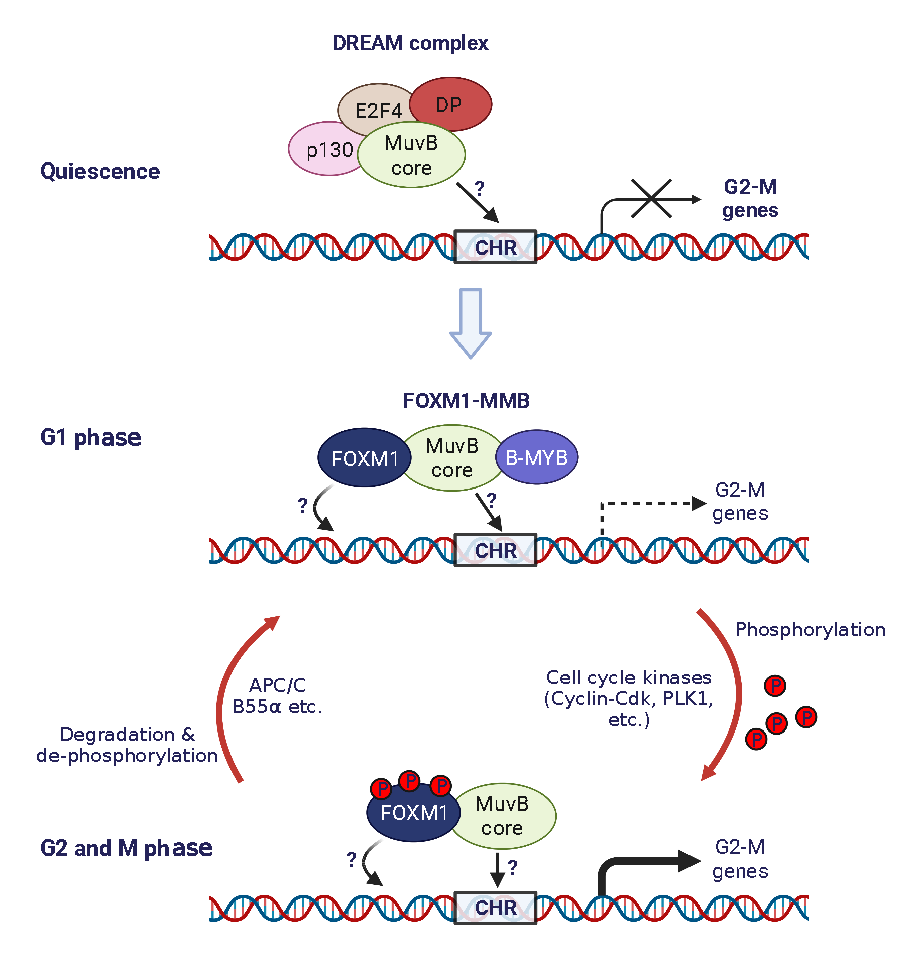
\includegraphics[width=0.85\textwidth]{chapter3/figures_foxm1/fig38.pdf}
    \caption[Model proposed for the cell cycle regulation by different protein complexes]{\textbf{Model proposed for the cell cycle regulation by different protein complexes.} The red Ps represent phosphorylation events. The question marks represent the uncertainty of DNA contacts. See more detailed description in the main text.}
    \label{fig:fig38}
\end{figure}

